\documentclass{article}
\usepackage{tikz}
\usetikzlibrary{matrix}
\begin{document}
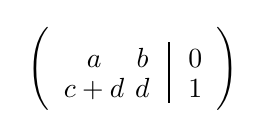
\begin{tikzpicture}
\matrix (m) [matrix of math nodes,left delimiter=(,right delimiter=),
  inner sep=2pt,outer sep=0pt]{
  a & b & [1em] 0 \\
  c +d & d & 1 \\ };
\draw ([xshift=0.5em]m-1-2.north east-|m-2-2.south east) -|
      ([xshift=0.5em]m-2-2.south east);
\end{tikzpicture}
\end{document}
